% !TEX root = ../../../main.tex
% 来源：中学数学实验教材·第一册（代数）
% 章节：因式分解与余式定理 / 余式定理及其推论
% 原始文件：5.tex，行 1722-1757
% 类型：tikz
% ---
    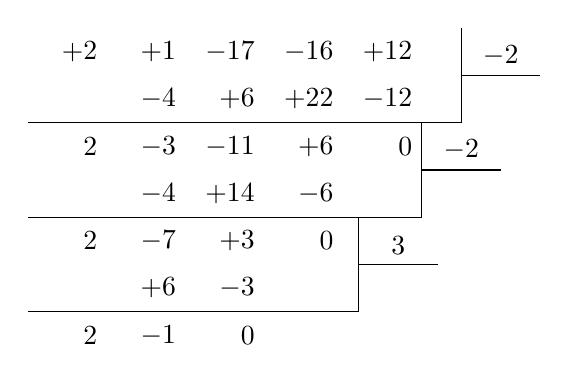
\begin{tikzpicture}[yscale=.6]
\foreach \x/\xtext in {0/2,1/-1,2/\boxed{0}}
{
    \node at  (\x,0)[left]{$\xtext$};
}        
\foreach \x/\xtext in {1/+6,2/-3}
{
    \node at  (\x,1)[left]{$\xtext$};
}  
\foreach \x/\xtext in {0/2,1/-7,2/+3,3/\boxed{0}}
{
    \node at  (\x,2)[left]{$\xtext$};
}  
\foreach \x/\xtext in {1/-4,2/+14,3/-6}
{
    \node at  (\x,3)[left]{$\xtext$};
}  
\foreach \x/\xtext in {0/2,1/-3,2/-11,3/+6, 4/\boxed{0}}
{
    \node at  (\x,4)[left]{$\xtext$};
}  
\foreach \x/\xtext in {1/-4,2/+6,3/+22, 4/-12}
{
    \node at  (\x,5)[left]{$\xtext$};
} 
\foreach \x/\xtext in {0/+2,1/+1,2/-17,3/-16, 4/+12}
{
    \node at  (\x,6)[left]{$\xtext$};
} 
\draw (-1,.5)--(3.2,.5)--(3.2,2.5)--(4,2.5)--(4,4.5)--(4.5,4.5)--(4.5,6.5);
\draw (-1,2.5)--(3.2,2.5);
\draw (-1,4.5)--(4,4.5);
\draw (3.2,1.5)--node[above]{3}(4.2,1.5);
\draw (4,3.5)--node[above]{$-2$}(5,3.5);
\draw (4.5,5.5)--node[above]{$-2$}(5.5,5.5);
 \end{tikzpicture}    
